\documentclass[11pt]{article}
\usepackage[margin=1in]{geometry}
\usepackage[T1]{fontenc}
\usepackage{lmodern}
\usepackage{amsmath,amssymb}
\usepackage{booktabs}
\usepackage{array}
\usepackage{graphicx}
\usepackage{xcolor}
\usepackage[numbers,sort&compress]{natbib}
\usepackage[hidelinks]{hyperref}
\graphicspath{{figures/}}

\title{Optimizing the Optimizers:\\ Measuring Learned Control of MIP Solvers on a Single DGX Spark}
\author{Berk Orbay\\ \small\texttt{berk.orbay@tideseed.com}\thanks{Experiments designed, run and written up with AgentRA (Agent Research Assistant; AgentRA is mainly Claude Opus 5.5), under the author's direction; every number was produced by the code and experiment definitions in the public repository
\url{https://github.com/berkorbay/optopt} and can be re-derived with \texttt{optopt reproduce}. A companion file for
automated readers is provided as an ancillary file and in the repository (Appendix~\ref{app:companion}). The study was reviewed, with suggestions for improvement, by Claude
Fable 5.1 (Anthropic) and OpenAI GPT-6 Astra (ChatGPT).}}
\date{Technical report --- 24 September 2026}

\begin{document}
\maketitle

\begin{abstract}
The default settings of a mixed-integer programming (MIP) solver are tuned to do well on average; a user with a fixed
time budget cares about the instance at hand. On one NVIDIA DGX Spark we measure, for HiGHS, SCIP and NVIDIA cuOpt,
how much sooner a good solution could be found by choosing settings per instance, whether that gain comes from the
initial choice or from switching settings during the solve, and what simple and learned controllers recover, with
their decision time charged to the budget. The measure is the primal integral, the gap to the best known solution
averaged over the budget. Over 8{,}000 runs on MIPLIB 2017, two ML4CO families and PGLib-UC unit commitment give
three main findings. First, choosing the best of six configurations per instance would lower the primal integral by
19\,\% over all 336 attempted instances, 25\,\% on the 313 where some configuration finds a solution and 41\,\% on
MIPLIB, measured with one seed. Second, inside SCIP most of this comes from the initial choice: the right static
setting is worth 12\,\% (45 instances) and 20\,\% (the 20 with the most headroom), while the six switching schedules
we tried add about 2\,\% at 120\,s and nothing detectable at 300\,s. Third, on held-out ML4CO instances one fixed
setting improves on SCIP's defaults by 33\,\%, and by 41\,\% when applied at the solver's first callback instead of
before presolve, which on load balancing avoids one start-up heuristic; an untrained local language-model agent makes the same first move in most runs, but the fixed
setting applied at that callback beats it on 22 of 30 instances. Running cuOpt beside HiGHS or SCIP, or passing
cuOpt's solutions into SCIP, gains 14--30\,\% with no model. The harness is released as a Python library with the
experiment definitions, and the original run trajectories as a versioned archive.
\end{abstract}

\section{Introduction}
Planners, schedulers and energy traders who use MIP solvers rarely wait for a proof of optimality. They need a good
solution within a fixed time, and how soon a solver finds one depends strongly on its settings.
Figure~\ref{fig:pi} shows an example. On the MIPLIB instance \texttt{h80x6320d}, SCIP with its default settings stays
62\,\% away from the best known solution for the first minute and then finds the optimum at 61\,s. The same solver
with cutting-plane separation switched off is within 8\,\% after two seconds but has not reached the optimum when the
120\,s run ends. The primal integral $P(T)$~\citep{berthold2013primal} turns such a curve into one number, the
average gap over the budget $T$, and so rewards finding good solutions early: here 0.318 for the default and 0.049
without separation.

\begin{figure}[t]\centering
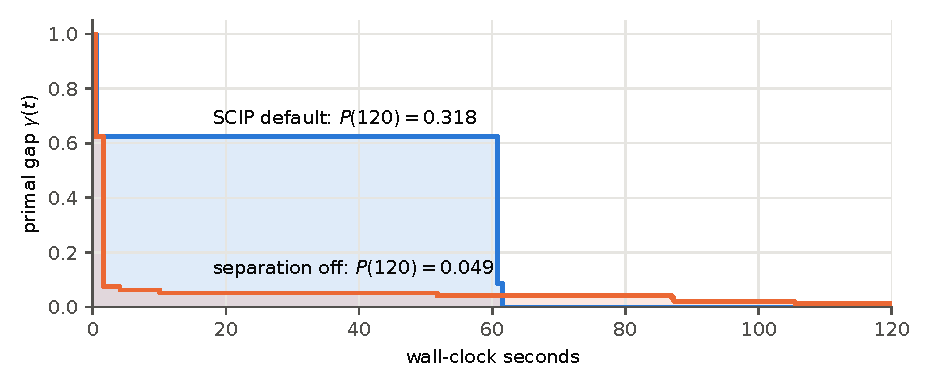
\includegraphics[width=0.9\linewidth]{fig_primal_integral.pdf}
\caption{The primal integral on one run each of SCIP's default and of SCIP with separation off (MIPLIB
\texttt{h80x6320d}, 120\,s, seed 0). The curve is the gap between the best solution found so far and the best known
solution; it is 1 until the first solution. $P(120)$ is the shaded area divided by 120\,s: lower is better.}\label{fig:pi}
\end{figure}

Two developments make such differences worth exploiting. GPU solvers such as cuOpt~\citep{cuopt} now run beside CPU
solvers on the same small machine, and agents --- from small learned models to language models --- can read a
solver's state and change its settings while it runs. This paper measures how much there is to gain, whether the gain
comes from the initial choice of settings or from changing them later, and which controllers recover it. All
measurements use the conditions a user faces: one machine, a wall-clock budget that includes the controller's own
decision time, and instances the controller has not seen.

\paragraph{Headroom.} We call \emph{headroom} the gain available from choosing a configuration per instance instead of
using one configuration for all. A small example: configuration A scores $P=0.2$ on instance 1 and 0.6 on instance 2;
configuration B scores 0.5 and 0.1. The best single configuration is B (mean 0.30, against 0.40 for A). An
\emph{oracle} that picks the better configuration for each instance scores 0.2 and 0.1 (mean 0.15). The headroom is
the oracle's improvement over the best single configuration: $(0.30-0.15)/0.30 = 50\,\%$. It bounds what any method
choosing among these configurations can gain; if one configuration were best everywhere, it would be zero. A solver's
result also varies from run to run with its random seed, and an oracle chosen and scored on the same run counts that
luck as headroom. Where a second seed exists (Sections~\ref{sec:switch} and~\ref{sec:agent}) the oracle therefore
chooses on one seed and is scored on another. The cross-solver headroom of Section~\ref{sec:headroom} uses one seed;
Section~\ref{sec:headroom} reports how much of it survives a second seed.

\paragraph{Contributions.}
\begin{enumerate}
\item \textbf{How much there is to gain.} Choosing per instance among six configurations of HiGHS, SCIP and cuOpt
  would lower the primal integral by 19\,\% over all attempted instances (25\,\% where some configuration finds a
  solution) and 41\,\% on MIPLIB, compared with the best single configuration (one seed); on a five-seed subset about
  80\,\% of the gain repeats (Section~\ref{sec:headroom}).
\item \textbf{Choosing versus switching.} Inside SCIP we split the gain into the part from choosing the right
  setting at the start and the part from changing settings during the solve (Figure~\ref{fig:decomp}). The initial
  choice is worth 12\,\% at 120\,s (45 instances) and 20\,\% at 300\,s (the 20 with the most headroom); the six
  switching schedules we tried add about 2\,\% and nothing detectable on the primal integral, and 1.5--1.6\,\% on
  the primal-dual integral (upper 95\,\% bounds 3.8--4.3\,\%). We have not found this split measured for MIP before (Section~\ref{sec:switch}).
\item \textbf{Agents measured on equal terms.} Every controller gets the same problem, solver and wall-clock budget,
  and its thinking time counts against the budget: the defaults, the best fixed setting, an online bandit, Laya, and
  local and hosted language models with and without Laya as a tool. A control that applies a fixed setting at the
  same callback as the agents shows that the language-model agent's advantage over the fixed setting comes from
  \emph{when} it acts: applied at that callback, the fixed setting beats the agent on 22 of 30 instances, and no
  benefit was detected from the agent's later decisions (Section~\ref{sec:agent}).
\item \textbf{Two solvers together.} Running cuOpt beside HiGHS improves on HiGHS alone by 30\,\%, and beside SCIP on
  SCIP alone by 21\,\% (44 instances); passing cuOpt's
  solutions into SCIP improves SCIP's own primal integral by 14\,\%. We report which solver interfaces allow this
  safely (Section~\ref{sec:parallel}).
\item \textbf{A reusable harness.} The Python library \texttt{optopt}: solver wrappers that record every solution
  and bound over time, an agent interface that charges decisions to the wall clock, an exact-arithmetic solution
  checker, the experiment definitions, the original run trajectories as a versioned archive, and
  \texttt{optopt reproduce}, which re-derives every table from them. It
  also records a pitfall for anyone measuring SCIP: when SCIP reports a new best solution, its primal bound still
  holds the previous one (Appendix~\ref{app:metrics}).
\end{enumerate}

\paragraph{Related work.} Learning for MIP is an established field~\citep{bengio2021ml,scavuzzo2024ml}, with learned
branching~\citep{khalil2016learning,gasse2019exact}, heuristics and diving~\citep{khalil2017heuristics,nair2020solving,
chmiela2021learning}, large-neighbourhood search~\citep{song2020general,sonnerat2021learning,huang2023searching}, cut
selection~\citep{tang2020rl,paulus2022learning,wang2023learning}, node selection~\citep{he2014learning,labassi2022nodes},
restarts~\citep{anderson2019restarts} and configuration~\citep{hutter2010mipconfig,valentin2022instance,li2025benloc}.
Per-instance algorithm selection and portfolios~\citep{rice1976algorithm,xu2008satzilla,xu2011hydramip,bischl2016aslib},
including selection among MIP solvers~\citep{lindauer2019oasc,szeider2026zerofolio}, online bandits inside or on top
of SCIP~\citep{hendel2019bandits,chmiela2023online,cai2025balans}, switching strategies during the
solve~\citep{diliberto2016dash,hendel2017phases,berthold2018phases}, racing solver copies~\citep{mexi2026rexi,
yilmaz2025parbalans} and language models that configure solvers~\citep{lawless2025llm,luo2026grimip,cai2025multitask,
pellegrino2025transformer} all exist; we use these methods and claim no novelty for them. What we add is a measurement
under a user's conditions: a CPU and GPU portfolio scored by the primal integral, the choosing-versus-switching split
for MIP (made for black-box optimisation by \citet{vermetten2020dynamic}), and very different agents compared on the
same budget with their thinking time charged. Appendix~\ref{app:related} details a structured search of about 180
works, including relevant work we could not read.

\section{Setup}\label{sec:setup}
\paragraph{Machine and solvers.} One NVIDIA DGX Spark (GB10: 10 Cortex-X925 and 10 Cortex-A725 cores, Blackwell GPU,
121\,GiB memory shared by CPU and GPU). HiGHS 1.15.1, SCIP 10.0 and cuOpt 26.08 from released wheels. Timed CPU runs
use one thread. In the SCIP experiments of Sections~\ref{sec:switch}--\ref{sec:parallel} each run is pinned to one
Cortex-X925 core with a hard memory cap; the cross-solver grid of Sections~\ref{sec:headroom} and~\ref{sec:predict} was
not pinned, so its runs moved between fast and slow cores (Appendix~\ref{app:resources}). Budgets are equal for the
solver; they do not equalise total compute: a local language-model server and cuOpt's host threads are extra.
\paragraph{Instances.} 80 MIPLIB 2017 benchmark instances~\citep{gleixner2021miplib}, at most one per MIPLIB group;
the ML4CO item-placement and load-balancing families~\citep{gasse2022ml4co}, trained on their official training
instances and tested on instances from their official validation split; and the 56 PGLib-UC unit-commitment
cases~\citep{pglibuc}, built with the benchmark's own formulation~\citep{knueven2020uc}. On 23 of the 24 FERC cases no
configuration finds a solution within 60\,s (Appendix~\ref{app:data}).
\paragraph{Metric.} The normalised primal integral $P(T)\in[0,1]$~\citep{berthold2013primal} (Figure~\ref{fig:pi}):
the relative gap between the best solution found so far and the best known value, averaged over the wall-clock budget
$T$, with the gap set to 1 until the first solution. The budget starts once the model has been read (median 1.8\,s,
at most 5.8\,s), except in the live two-solver runs of Section~\ref{sec:parallel}, where it starts when both processes
are launched and so includes reading the model. The primal-dual integral (PDI) uses the solver's own bound in place of the best known value, so it
also rewards progress on the bound. The final solution of every SCIP run, and of the HiGHS and cuOpt runs in the
two-solver experiments, is checked independently against the model; earlier solutions that enter $P(T)$ are not
checked (Appendix~\ref{app:metrics}).
\paragraph{Protocol.} Where two seeds exist, oracles choose on one seed and are scored on another; the cross-solver
grid has one seed (Section~\ref{sec:headroom}). Learned selectors are evaluated by grouped
cross-validation: ML4CO by its official split, PGLib-UC by power system; a second scheme leaves a whole family out.
Paired tests are over instances, with the seeds of an instance averaged. The machine was shared with other work, and
results shift between sessions: the same two arms on the same 60 runs scored 0.7--2.7\,\% worse on the second day than
on the first. We therefore compare arms within one session and treat differences below about 3\,\% between sessions
as noise. Within a session, arms ran in a fixed order per instance, not randomised, so slow drift within a session is
not excluded. Only the 10\,\% headroom threshold of Section~\ref{sec:headroom} was set in advance. We name choosing
versus switching (Section~\ref{sec:switch}) and the timing-matched control (Section~\ref{sec:agent}) as the principal
comparisons after the fact, to guide reading; like all others they are exploratory, not pre-registered.

\section{How much is there to gain?}\label{sec:headroom}
Six configurations --- default and primal-focused variants of HiGHS, SCIP and cuOpt (Table~\ref{tab:portfolio}) ---
were run on all 336 instances. Choosing per instance would lower the primal integral by 19\,\% over all of them and
by 41\,\% on MIPLIB (Table~\ref{tab:headroom}), above the 10\,\% threshold we set before any run. On 23 unit-commitment
cases, all from the FERC system, no configuration finds a solution within 60\,s, so every configuration scores $P=1$
there; on the 313 instances where at least one configuration finds a solution the headroom is 25\,\%. The selectors of
Section~\ref{sec:predict} are trained and evaluated on those 313, which include one FERC case. This oracle is chosen
and scored on the same seed. On a 12-instance MIPLIB subset run with five seeds and the four CPU configurations, a
held-out oracle realises 26.3\,\% of an apparent 31.8\,\%, that is 83\,\% (Table~\ref{tab:variance}); cuOpt was not
re-run with extra seeds. These runs were not pinned to cores, so a run's effective budget varied by up to a factor of
two, which inflates single-seed headroom. cuOpt's solutions are feasible at its own tolerance of $10^{-4}$; two of 140
checked exceed $10^{-6}$ (Appendix~\ref{app:metrics}). No configuration wins everywhere: HiGHS with more
heuristics, or SCIP's default, is the best fixed choice where the CPU solvers finish, while cuOpt wins at short
budgets and on the MIPLIB instances that neither CPU solver finishes in 300\,s (Appendix~\ref{app:trackA}).
\begin{table}[t]\centering\small
\begin{tabular}{lrrlrrrr}
\toprule
 & \multicolumn{2}{c}{instances} & & & \multicolumn{2}{c}{oracle headroom} \\
family & all & some sol. & budget & best fixed & $P$ (all) & all & some sol. \\
\midrule
MIPLIB 2017 & 80 & 80 & 60\,s & H1 & 0.337 & 41\% & 41\% \\
ML4CO item placement & 100 & 100 & 30\,s & H1 & 0.207 & 16\% & 16\% \\
ML4CO load balancing & 100 & 100 & 30\,s & S0 & 0.067 & 15\% & 15\% \\
PGLib-UC & 56 & 33 & 60\,s & C0 & 0.788 & 5\% & 11\% \\
Pooled & 336 & 313 & 30\,s & H1 & 0.327 & 19\% & 25\% \\
\bottomrule
\end{tabular}
\caption{Headroom across HiGHS, SCIP and cuOpt (six strategies, Table~\ref{tab:portfolio}): normalised primal integral $P$ of the best fixed strategy and the improvement a per-instance oracle would achieve, one seed. \emph{All}: every attempted instance, with $P=1$ for every strategy where none finds a solution (23 PGLib-UC cases, all from the FERC system). \emph{Some sol.}: instances where at least one strategy finds a solution; the selectors of Section~\ref{sec:predict} are trained and evaluated on this cohort. On a five-seed MIPLIB subset about 80\,\% of the single-seed headroom repeats (Appendix~\ref{app:trackA}).}\label{tab:headroom}
\end{table}

\section{Predicting the right configuration}\label{sec:predict}
The most direct way to recover the headroom is to predict the right configuration from the instance before solving
it. We trained three selectors on 62 features of the instance's constraint matrix: LightGBM, a small neural network
(MLP) and Laya~\citep{laya2026}, a 421M-parameter decision model (a ModernBERT-large
encoder~\citep{warner2025modernbert} with a classification head) that reads the features as text. Laya was used both
untrained and fully fine-tuned, with training targets that give each configuration a weight falling with its cost,
$P(a)\propto\exp(-\beta\,\mathrm{cost}_a)$. Table~\ref{tab:selection} reports the share of the headroom each selector
recovers: 0 means no better than the best single configuration, 1 means as good as the oracle.

At 10\,s, fine-tuned Laya recovers 31\,\% of the headroom (95\,\% interval 14--48\,\%, the only interval that excludes
zero) and LightGBM 24\,\%. Compared directly on the same test instances, no superiority was established: the difference is
$+0.07$ of the headroom (interval $-0.13$ to $+0.34$, paired Wilcoxon $p=0.67$) at 10\,s and $+0.06$ ($p=0.09$) at
30\,s. On a family left out of training the difference is clear: at 30\,s Laya stays level with the best fixed
configuration while LightGBM and the MLP fall about 0.4 below it, and Laya beats LightGBM by 0.37 of the headroom
(interval 0.16 to 0.68, $p<10^{-4}$). These intervals hold the fitted models fixed; they do not cover retraining or
other folds. The pooled result comes mostly from MIPLIB. Averaged per family instead, every selector falls below each
family's best fixed configuration at 10\,s, mainly because of unit commitment, where the headroom is small and a wrong
choice costs more than a right one gains; at 30\,s only Laya stays above it (Appendix~\ref{app:trackA}). Laya answers
in 30--56\,ms (median, two measurements) and, called every few seconds, does not measurably slow cuOpt on the shared GPU
(Appendix~\ref{app:contention}). Computing the features takes 0.3\,s (median; at most 5.2\,s); this is not charged to
the budget and would matter at 10\,s, so the 10\,s results assume the features are already computed. With these
features and models, prediction before the solve recovers part of the headroom and leaves the rest.
\begin{table}[t]\centering\small
\begin{tabular}{lrrrr}
\toprule
& \multicolumn{2}{c}{seen families (pooled)} & \multicolumn{2}{c}{unseen family (LOFO)} \\
policy & 10\,s & 30\,s & 10\,s & 30\,s \\
\midrule
Best fixed, chosen on training data & +0.00 & +0.00 & -1.09 & +0.00 \\
LightGBM & +0.24 & +0.03 & -0.03 & -0.40 \\
MLP & +0.07 & -0.00 & -0.08 & -0.42 \\
Laya, zero-shot & -0.37 & -0.57 & -1.04 & -1.38 \\
Laya, fine-tuned & +0.31 & +0.10 & +0.09 & -0.02 \\
Oracle & +1.00 & +1.00 & +1.00 & +1.00 \\
\bottomrule
\end{tabular}
\caption{Selecting a strategy before the solve from 62 static instance features: closed gap between the hindsight single best strategy (0) and the oracle (1); one model for all families, 163 instances with grouped cross-validation (seen families) and 313 with leave-one-family-out (unseen family), all from the cohort where some strategy finds a solution (one FERC unit-commitment case). The hindsight single best defines 0; the best fixed strategy chosen on the training folds can score below it. Intervals resample test instances with the fitted models held fixed; they do not cover retraining or other folds. Positive closed gaps whose 95\,\% interval excludes zero: the fine-tuned Laya, seen families, 10\,s ([0.14, 0.48]); intervals, per-family results and time-to-target are in Appendix~\ref{app:trackA}.}\label{tab:selection}
\end{table}

\section{Choosing versus switching}\label{sec:switch}
A controller could also change settings during the solve. Inside SCIP we compared six static settings (default,
separation off, pseudo-cost branching, inference branching, heuristics off, aggressive heuristics) with six schedules
that switch between them or restart the search, either at 25\,\% of the budget or after 20\,\% of the budget without
progress. All twelve ran on 45 MIPLIB instances that SCIP does not solve quickly, with two seeds (Table~\ref{tab:b2}).
Each choice is made on one seed and scored on the other, in both directions, averaged. Let $B$ be the mean cost of the
single static setting that is best on average, $S$ the mean cost when each instance gets its own best static setting,
$A$ the same with all twelve arms (schedules included) available, and $R$ the mean cost when each run gets the arm
that won that very run ($R$ is hindsight, not chosen on the other seed). We report
\begin{itemize}
\item \emph{choosing}: $(B-S)/B$, the gain from the best static setting per instance;
\item \emph{switching}: $(S-A)/B$, what the schedules add on top of that choice;
\item \emph{gap to the per-run hindsight oracle}: $(A-R)/B$, what knowing each run's winner in advance would add.
  It includes seed-to-seed noise, the limits of choosing on one seed, and anything the tested choices do not use.
\end{itemize}

Figure~\ref{fig:decomp} shows the result. At 120\,s, choosing is worth 11.8\,\% on $P$ and 6.5\,\% on PDI, and the
six schedules add 2.1\,\% and 1.6\,\% (upper 95\,\% bounds 7.3\,\% and 3.8\,\%). At 300\,s, on the 20 instances with the
most headroom, choosing is worth 20.4\,\% on $P$ and 11.3\,\% on PDI, while the schedules add $-0.2\,\%$ on $P$ and
1.5\,\% on PDI (interval $-0.2$ to 4.3\,\%). With these settings, schedules, instances and budgets, a controller gains
by choosing well at the start; the six schedules add little that transfers to a new seed. Other schedules, other actions or budgets beyond 300\,s may
still gain from switching: DASH~\citep{diliberto2016dash} gains by switching the branching rule at individual nodes, scored by time to
optimality, and Balans~\citep{cai2025balans} by switching large-neighbourhood operators.

\begin{figure}[t]\centering
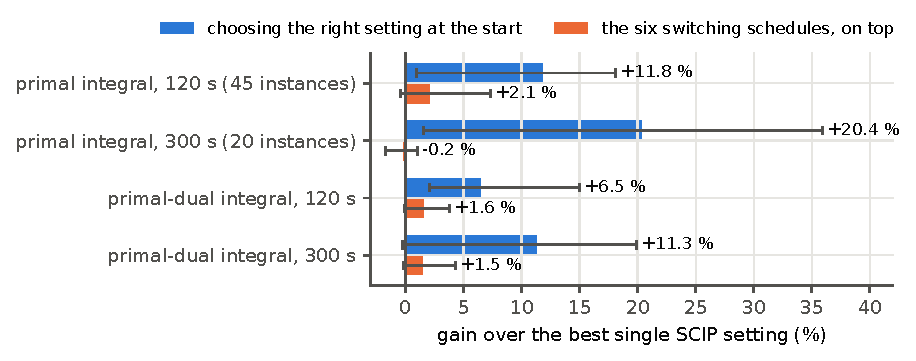
\includegraphics[width=0.9\linewidth]{fig_decomposition.pdf}
\caption{Where the gain inside SCIP comes from: choosing the right static setting per instance (blue) versus
switching settings during the solve on top of that choice (orange), both relative to the best single SCIP setting and
measured on a held-out seed. 120\,s: 45 MIPLIB instances; 300\,s: the 20 with the most headroom.}\label{fig:decomp}
\end{figure}

The gap to the per-run hindsight oracle is large. With five seeds, the setting that wins on one seed is also the
winner averaged over seeds in only 71\,\% of runs for $P$ (69\,\% for PDI). The tested predictors do not capture this
part; running several copies at once does (Section~\ref{sec:parallel}).
\begin{table}[t]\centering\small
\resizebox{\linewidth}{!}{\begin{tabular}{lrrrrr}
\toprule
& static choice & switching, on top & run-level (hindsight) & same winner & best static \\
\midrule
primal integral $P(120)$ & +11.8\% [+1.0, +18.1] & +2.1\% [-0.4, +7.3] & 5.0 pts & 56\% & INF \\
primal-dual integral PDI$(120)$ & +6.5\% [+2.1, +15.0] & +1.6\% [-0.1, +3.8] & 3.7 pts & 47\% & PSC \\
\bottomrule
\end{tabular}}
\caption{Choosing versus switching inside SCIP: SCIP~10 with six static settings (default, separation off, pseudo-cost branching, inference branching, heuristics off, aggressive heuristics) and six mid-solve schedules (restart at 25\,\% or after a 20\,\% stall, branching switches, heuristic bursts), 45 MIPLIB instances, 120\,s, two seeds, one run per Cortex-X925 core. Gains are over the best single static setting; choices made on one seed and scored on the other; 95\,\% bootstrap intervals. Run-level: additional gain of an oracle that sees the run itself.}\label{tab:b2}
\end{table}

\section{Agents in the loop}\label{sec:agent}
The end-to-end experiment gives an agent a problem, SCIP, a 120\,s wall-clock budget and one Cortex-X925 core with
8--9\,GiB of memory. SCIP starts with its default settings and calls the agent at solver events (a new best solution
or a solved node): first at the first such event after the start, then at the first event after each decision
interval. At each call the agent may keep the current setting, change it, or restart the search. SCIP's time limit is
wall-clock time, so the agent's thinking time is taken from the solver's budget (Appendix~\ref{app:agents}). Instance
features are computed before the start and not charged (median 0.3\,s, at most 5.2\,s).

On held-out ML4CO test instances, every agent whose first move is sensible recovers much of the headroom
(Table~\ref{tab:agent}). An online bandit with no training (UCB1 over the six settings) improves on the defaults by
21--27\,\%, and on item placement by about 30\,\%, better in 28 of 30 runs. The best fixed setting learned from 60
training instances (aggressive heuristics, one setting for both families) gives $+29\,\%$; LightGBM predicting a setting per
instance $+23\,\%$; a bandit that starts from that prediction $+29\,\%$; and Laya, fine-tuned for the same first
choice, $+28\,\%$: it learns to pick aggressive heuristics, the same choice as the best fixed setting.
\begin{table}[t]\centering\small
\setlength{\tabcolsep}{4pt}\begin{tabular}{lrrrrrr}
\toprule
 & & \multicolumn{2}{c}{agents} & \multicolumn{2}{c}{fixed from $t=0$} & 2 copies \\ instances $\times$ seeds & default & bandit & rules & aggr.\ heur. & sep.\ off & (2 cores) \\
\midrule
ML4CO, set 1 ($20\times2$) & 0.156 & 0.122 & 0.160 & -- & -- & 0.118 \\
MIPLIB ($15\times2$) & 0.390 & 0.383 & 0.401 & -- & -- & 0.374 \\
ML4CO set 2, item placement ($15\times2$) & 0.356 & 0.250 & -- & 0.245 & 0.304 & -- \\
ML4CO set 2, load balancing ($15\times2$) & 0.036 & 0.038 & -- & 0.035 & 0.041 & -- \\
\bottomrule
\end{tabular}
\caption{Agent in the loop: primal integral $P(120)$ (lower is better) of agents that start from SCIP's defaults in a fixed slice (one Cortex-X925 core, 9\,GiB, 120\,s wall clock including every agent decision). ML4CO instances are held out, from the validation split. Set 1: bandit deciding every 10\,s; set 2: every 5\,s. Significance tests in Appendix~\ref{app:agents}.}\label{tab:agent}
\end{table}

\paragraph{Language-model agents.} We gave the same task to two language models: Ornith-1.5-35B-A3B run locally
(NVFP4 on vLLM, thinking off), called every 20\,s, and OpenAI GPT-6 Luna through a ChatGPT Plus subscription
(reasoning effort low), called every 30\,s. Each call shows the model the same 62 features that Laya and LightGBM see,
SCIP's current state (elapsed time, gap, recent solutions, node rate, current setting, the model's own earlier
decisions) and the six settings with a one-line description each, and asks for one action.

\paragraph{When the agent acts.} A fixed setting is applied before SCIP starts, so it also governs presolve. An agent
can act only when SCIP first calls it: presolve takes about 0.25\,s on these instances, and the first call comes at a
median 0.35\,s (at most 1.1\,s), while SCIP is solving the root node. Part of an agent's advantage could therefore come
from \emph{when} it acts rather than \emph{what} it chooses. Table~\ref{tab:timing} separates the two. In one session,
on 30 held-out ML4CO instances with two seeds, it runs the defaults, aggressive heuristics set before presolve (the
best fixed setting on the training instances, one setting for both families),
the same setting applied by a fixed agent at the first call, the local language-model agent, and that agent's first
decision alone. Against the defaults these arms gain 33.3\,\%, 40.6\,\%, 34.3\,\% and 31.8\,\%.
\begin{itemize}
\item \emph{Timing.} Applying aggressive heuristics at the first call instead of before presolve is better on 24 of 30
  instances ($p=0.005$). The median per-instance gain is 12.7\,\% and the mean gain 10.9\,\%; a few instances lose
  heavily, so the 95\,\% bootstrap interval of the mean ($-3.9$ to $+22.3\,\%$) includes zero. The consistent part is on
  load balancing: better on 15 of 15 instances ($p<10^{-4}$), although $P$ only moves from 0.037 to 0.032; there the
  setting applied before presolve scores the same as the defaults. On item placement, 9 instances are better and 6
  worse ($p=0.25$).
\item \emph{Language-model agent versus the callback-fixed control.} Against the fixed setting applied at the same
  callback, the agent is worse on 22 of 30 instances ($p=0.004$): 10.6\,\% in the mean (interval $-18.9$ to $-4.0\,\%$) and 3.4\,\% at the median,
  mostly on item placement (worse on 12 of 15 instances, $p=0.03$). Its
  first move is aggressive heuristics in 49 of 60 runs and ``keep the defaults'' in the rest. This is an end-to-end
  comparison: it includes the agent's inference time (1.3\,\% of the budget) and its later actions, not only the
  quality of its choices.
\item \emph{Steering.} No benefit was detected from its later decisions: $+3.6\,\%$ over its first decision alone,
  with an interval ($-10.2$ to $+15.7\,\%$, $p=0.67$) that allows a sizeable gain or loss.
\item Against the fixed setting applied before presolve, the agent is not significantly different ($+1.5\,\%$,
  $p=0.31$).
\end{itemize}
On these two families the language model makes a good first choice without training. It matches the fixed setting
applied before presolve, and the same fixed setting applied at the agent's own first callback beats it.
\begin{table}[t]\centering\small
\begin{tabular}{@{}>{\raggedright\arraybackslash}p{0.50\linewidth}rr@{}}
\toprule
arm & $P(120)$ & vs defaults, 95\,\% interval \\
\midrule
SCIP defaults & 0.179 & -- \\
aggressive heuristics, set before presolve & 0.119 & $+33.3$\,\% $[+24.6, +41.4]$ \\
aggressive heuristics, set at the first solver event & 0.106 & $+40.6$\,\% $[+31.6, +48.0]$ \\
LLM agent, first decision only & 0.122 & $+31.8$\,\% $[+22.5, +41.2]$ \\
LLM agent, every 20\,s & 0.117 & $+34.3$\,\% $[+24.8, +42.2]$ \\
\midrule
\emph{contrast} (first vs second arm) & mean (median) & 95\,\% interval, $p$ \\
\midrule
timing: heuristics at first event vs heuristics before presolve & $+10.9$\,\% ($+12.7$) & $[-3.9, +22.3]$, $p=0.0047$ \\
judgement: LLM every 20\,s vs heuristics at first event & $-10.6$\,\% ($-3.4$) & $[-18.9, -4.0]$, $p=0.004$ \\
steering: LLM every 20\,s vs LLM first decision & $+3.6$\,\% ($-0.2$) & $[-10.2, +15.7]$, $p=0.67$ \\
first move: LLM first decision vs heuristics at first event & $-14.8$\,\% ($-2.7$) & $[-29.2, -3.6]$, $p<10^{-6}$ \\
replication: LLM every 20\,s vs heuristics before presolve & $+1.5$\,\% ($+5.6$) & $[-12.8, +13.2]$, $p=0.31$ \\
\bottomrule
\end{tabular}
\caption{Timing-matched controls, the primary agent comparison: 30 held-out ML4CO instances (validation split), two seeds, 120\,s, all arms in one session. Gains in primal integral, positive when the first arm is better: the gain in the mean, and in parentheses the median per-instance gain. Intervals: instance-level bootstrap of the mean gain; $p$: Wilcoxon signed-rank over instances. ``Heuristics'': the aggressive-heuristics setting; ``first event'': the first eligible solver event, where the agents first act.}\label{tab:timing}
\end{table}

\paragraph{Why the timing matters.} A follow-up session on the same 30 instances (one seed; Table~\ref{tab:timingmech}
in Appendix~\ref{app:agents}) applied aggressive heuristics before presolve, at the first call, and at the first call
after 10\,s, and recorded SCIP's statistics. On load balancing SCIP stays at the root node for the whole budget in
every arm, spends about 96 of the 120\,s in primal heuristics (almost all in RENS) and finds the same solutions in
every arm. The arms differ only at the start. Set before presolve, the setting also runs SCIP's zero-objective
heuristic at the start of the solve (0.59\,s on average), which delays the first solution from 0.73\,s to 1.25\,s.
Until the first solution the gap counts as 1, so this delay alone costs about $0.5/120\approx0.004$ in $P$, the whole
difference between the arms (0.035 against 0.031). Applied at the first call the setting again wins on 15 of 15
instances, and applied after 10\,s on 14 of 15. On item placement, where the first solution comes within 0.02\,s, the
arms do not differ significantly (11 better, 4 worse, $p=0.36$). The timing effect is therefore specific: one early
heuristic that the setting adds only when it is set before the solve, on instances whose first solution takes about a
second. It does not show that acting after presolve is better in general.

\paragraph{Other agents (first session).} Table~\ref{tab:llm} comes from an earlier session on the same 30 instances
and adds arms that Table~\ref{tab:timing} lacks. Laya as the agent, fine-tuned for the first choice, improves on the
defaults by 37.0\,\% and uses 0.1\,\% of the budget. Adding Laya's probabilities to the local model's prompt did not
improve it ($+34.6\,\%$). GPT-6 Luna improved on the defaults by 25.3\,\% (one seed); its decisions took a median
3.3\,s each, 10\,\% of the budget. In that session the local model scored $+37.5\,\%$ and the fixed setting before
presolve $+31.7\,\%$; Table~\ref{tab:timing} replicates both at $+34.3\,\%$ and $+33.3\,\%$, so arms are compared only
within one table. On the primal-dual integral all agents in Table~\ref{tab:llm} are within 3\,\% of each other, and
their differences come from the 15 item-placement instances: on load balancing every arm of that table scores
0.035--0.038.
\begin{table}[t]\centering\small
\begin{tabular}{lrrrrr}
\toprule
arm & runs & $P(120)$ & vs default & vs best fixed & thinking \\
\midrule
SCIP defaults (no agent) & 60 & 0.184 & -- & -46.3\,\%$^{*}$ & -- \\
best fixed setting from training & 60 & 0.126 & +31.7\,\%$^{*}$ & -- & -- \\
Laya as the agent (fine-tuned, $t=0$) & 60 & 0.116 & +37.0\,\%$^{*}$ & +7.9\,\% & 0.1\,\% \\
LLM agent: Ornith-1.5-35B-A3B & 60 & 0.115 & +37.5\,\%$^{*}$ & +8.5\,\% & 1.3\,\% \\
LLM agent + Laya as a tool & 60 & 0.121 & +34.6\,\%$^{*}$ & +4.3\,\% & 1.5\,\% \\
LLM agent: GPT-6 Luna (hosted) & 30 & 0.137 & +25.3\,\%$^{*}$ & -15.3\,\% & 10.1\,\% \\
\bottomrule
\end{tabular}
\caption{The end-to-end agent experiment with LLM agents: 30 held-out ML4CO instances (validation split), SCIP starting from its defaults, one Cortex-X925 core and 8\,GiB, 120\,s of wall clock that includes every model call; two seeds (the hosted model one). Ornith-1.5-35B-A3B runs locally (NVFP4 on vLLM, thinking off) and is asked every 20\,s; GPT-6 Luna (ChatGPT Plus, reasoning effort low) every 30\,s. Gains in primal integral; $^{*}$ paired Wilcoxon $p<0.05$. \emph{Thinking}: share of the budget spent waiting for the agent.}\label{tab:llm}
\end{table}

\section{Two solvers at once}\label{sec:parallel}
Run-to-run variation can be used without any prediction by running solvers side by side and keeping the better
solution at each moment~\citep{gomes2001portfolios,mexi2026rexi}. On a machine with a GPU the natural pair is a CPU
solver and a GPU solver. Estimated from separately recorded runs, HiGHS on one thread plus cuOpt would capture 80\,\%
of the headroom between solvers on the instances where some configuration finds a solution (Table~\ref{tab:parallel}).
Run live on the 80 MIPLIB instances at 60\,s, launched together, with both arms of each comparison interleaved in one
session in a fixed order per instance, and the clock started at launch:
\begin{itemize}
\item HiGHS on one core with cuOpt on the GPU improves on HiGHS alone by 30.4\,\% (95\,\% interval 17.7 to 44.2\,\%;
  better on 61 instances, worse on 13, $p<10^{-8}$);
\item SCIP with cuOpt improves on SCIP alone by 21.5\,\% (interval 9.3 to 36.9\,\%; better on 28, worse on 13,
  $p<10^{-4}$) on the first 44
  instances in job-file order; this run stopped at the end of its scheduled window.
\end{itemize}
Scores use each solver's best solution; cuOpt's are feasible at its own tolerance of $10^{-4}$, and two of the 140
checked exceed $10^{-6}$ (Appendix~\ref{app:metrics}).
Within SCIP, two copies with different seeds improve $P$ by 7\,\% and PDI by 5.5\,\%. Each of these uses more compute
than a single run: cuOpt adds the GPU and five host cores.

The two solvers can also exchange solutions. When cuOpt's solutions are passed to SCIP through SCIP's heuristic
interface, SCIP's own primal integral improves by 14\,\% ($p<10^{-3}$; better on 47 instances, worse on 24). This
matters when one solver's result is needed together with its bound. The pair's best-of value does not improve beyond
the plain race, because cuOpt already held those solutions. Passing SCIP's solutions to cuOpt as well costs 15\,\%:
cuOpt switches off its presolve once it accepts outside solutions. Appendix~\ref{app:nofruit} describes the interfaces,
including one that crashes SCIP.
\begin{table}[t]\centering\small
\begin{tabular}{llrr}
\toprule
setting & portfolio & $P$ gain & PDI gain \\
\midrule
HiGHS/SCIP/cuOpt study, pooled (313 inst.) & HiGHS (1 thread) $\|$ cuOpt (GPU) & 22\,\% & -- \\
SCIP, 20 MIPLIB inst., 120\,s & 2 copies of the best setting & 7\% & 5\% \\
SCIP, 20 MIPLIB inst., 120\,s & 3 copies of the best setting & 9\% & 8\% \\
SCIP, 20 MIPLIB inst., 120\,s & 5 copies of the best setting & 11\% & 9\% \\
\bottomrule
\end{tabular}
\caption{Parallel portfolios, computed exactly from recorded trajectories: best incumbent (and bound) of runs executed side by side, against the best single strategy. HiGHS$\|$cuOpt captures 80\,\% of the cross-solver oracle headroom; SCIP copies differ only in the random seed.}\label{tab:parallel}
\end{table}

\section{Discussion}
\paragraph{What this means in practice.} For a user with a time budget, within the families, hardware and budgets
(30--300\,s) we tested:
\begin{enumerate}
\item Run a GPU solver beside the CPU solver: $+30\,\%$ over HiGHS alone and $+21\,\%$ over SCIP alone (44 instances), with no model.
\item Choose the setting once, at the start. On these ML4CO families one fixed setting chosen on training instances,
  and a fine-tuned Laya, improve on SCIP's defaults by about a third; an untrained local language model finds the same
  first move but does not beat the fixed setting applied at the same callback. Where the first solution takes about a
  second, check whether a setting adds work before it: on load balancing, aggressive heuristics set before the solve
  delayed the first solution by half a second.
\item If one solver's result is needed, pass the other solver's solutions in through the supported heuristic
  interface ($+14\,\%$).
\end{enumerate}
For learned controllers such as Laya, the useful task is therefore to diagnose the instance early, measured against
the best fixed setting and an online bandit, rather than to steer the solver continuously.

\paragraph{Future research.} (i) A new test cohort from families where no single setting is best on the training
data, with the protocol and one primary comparison fixed in advance and the timing-matched controls as baselines.
(ii) A short diagnostic run, charged to the budget, before a single choice, with a rule to keep the default when the
predicted gain is small; and richer state (root LP statistics, early solutions) for learned selectors. (iii) Budgets
longer than 300\,s, with a small set of schedules fixed in advance. (iv) Language-model agents with an explicit
thinking-time budget that decide \emph{when} to act, not only what to do. (v) Which solvers to run or pair under a
compute budget, with CPU, GPU, memory and energy counted, and exchange in both directions with HiGHS as the CPU
partner. (vi) Using the GPU \emph{inside} a MIP solver: GPU LP solvers of the PDLP type for relaxations in a CPU
branch-and-bound, and GPU heuristic populations. These are solver-engineering projects, and several GPU jobs at once
need scheduling: two slowed each other in our measurements (Appendix~\ref{app:contention}).

\paragraph{Limitations.} All timings come from one DGX Spark. Whether the conclusions transfer to other hardware is
untested: relative results can change with the balance of CPU and GPU and with memory contention. SCIP is the only solver studied in depth, the action sets are small and hand-picked, most results
use two seeds, the language-model agents saw two instance families, and budgets are at most 300\,s. Tests are paired
over instances (seeds averaged). Apart from the 10\,\% headroom threshold set in advance, the comparisons are
exploratory rather than pre-registered, including the principal ones named in Section~\ref{sec:setup}. An interval that includes zero
is not evidence that two arms are equal, so we report its bounds. Only final solutions are checked independently. Instance features are computed before the clock starts (Appendix~\ref{app:limitations}).

\section{Conclusion}
In HiGHS, SCIP and cuOpt, choosing settings per instance could lower the primal integral by 19\,\% over all attempted
instances and 25\,\% where some configuration finds a solution (one seed; about 80\,\% of it repeats on a five-seed
subset), and inside SCIP most of it comes from the initial choice rather than from the switching schedules we tried.
Running cuOpt beside HiGHS recovers 30\,\% and beside SCIP 21\,\% (44 instances) with no model. One fixed setting chosen on training instances
improves on SCIP's defaults by a third on the ML4CO families; an untrained local language model finds the same first
move, but the fixed setting applied at the same callback beats it on 22 of 30 instances. Two questions remain open:
whether an agent can beat the right fixed choice on families where that choice is not obvious, and whether switching
helps at budgets beyond 300\,s. The library, the experiment definitions, the archived trajectories and
\texttt{optopt reproduce} are released so that both can be tested against the same baselines.

\bibliographystyle{plainnat}
\bibliography{refs}

\appendix
\paragraph{Naming.} The appendix and the repository call the cross-solver study (HiGHS, SCIP, cuOpt; Sections~\ref{sec:headroom},
\ref{sec:predict} and \ref{sec:parallel}) \emph{Track~A}, and the SCIP studies (Sections~\ref{sec:switch} and
\ref{sec:agent}) \emph{Track~B}, with B0--B3 its experiments.

\section{Related work in detail, and work behind paywalls}\label{app:related}
We searched for prior work that uses a learned, neural or foundation model for the solver-side functions studied here
(per-instance configuration, switching during the solve, selection across solvers), in four sweeps: branching and node
selection; primal heuristics and large-neighbourhood search; configuration, selection and dynamic control; and LLMs,
foundation models and GPU solvers (159 works), followed by a re-check of the novelty claims (21 more; the notes, with the evidence for each entry, are in the repository vault
under \texttt{40-literature/prior-art}). Learned per-instance configuration of one solver is well
established~\citep{xu2011hydramip,valentin2022instance,li2025benloc}; BenLOC's finding that learned gains over the
per-dataset best stay under 5\,\% and that tree models beat deep ones agrees with our Table~\ref{tab:selection}. The
closest foundation-model work, GRIMIP~\citep{luo2026grimip}, reports primal-dual integrals on the same ML4CO families
and MIPLIB, but tunes Gurobi with about ten solver runs per instance; our selectors make one prediction inside the
budget. Choosing among SCIP settings per instance from features was studied by \citet{georges2018selection}, and
choosing among MIP solvers (CBC, CPLEX, Gurobi, SCIP, Xpress) is the ASlib MIP-2016 scenario of the 2017 selection
competition, where the best selector closed about half of the gap to the oracle~\citep{lindauer2019oasc}. What we did
not find --- a GPU solver in the portfolio, the primal integral as the selection target, a fine-tuned pretrained encoder
as the selector --- rests on negative searches in which part of the 2025--2026 preprint literature could only be
reached by web search, so we make no priority claim. Relevant works we could not read legally are listed separately in Appendix~\ref{app:paywalled}.

\subsection{Paywalled research}\label{app:paywalled}
This subsection is the only place in the paper that cites work we could not read. The following works appear relevant but are behind publisher paywalls, and we
found no legal free copy (preprint, accepted manuscript, repository or thesis version). \emph{We have not read them in
full.} They were found through accessible papers that cite or describe them, or judged relevant from their abstract
and metadata; the descriptions below are limited to what those sources state. Per-instance configuration by clustering
(ISAC,~\citealp{kadioglu2010isac}) and algorithm selection combined with a schedule of short runs
(3S,~\citealp{kadioglu2011threes}); running differently configured copies of one MILP solver in parallel with shared
information~\citep{carvajal2014diversification}; learned per-instance decisions inside a solver, whether to use a
decomposition~\citep{kruber2017decomposition} or whether CPLEX should linearise a quadratic
problem~\citep{bonami2018miqp}; SCIP's non-learned combination of branching scores~\citep{achterberg2009hybrid}; a
survey of learning for branching~\citep{lodi2017survey}; and the standard account of performance variability under
seeds~\citep{lodi2013variability}, which underlies the parallel copies of Table~\ref{tab:parallel}. Where a work in this
paper is paywalled but a legal preprint exists, the bibliography points to the preprint.

\section{Hardware, software and resources}\label{app:resources}
{\sloppy All experiments ran on one NVIDIA DGX Spark: GB10 Grace--Blackwell superchip (10 Cortex-X925 + 10 Cortex-A725
cores, Blackwell GPU, 128\,GB coherent unified memory, of which the operating system reports 121\,GiB), Ubuntu 24.04, kernel 6.17, driver 580.173.02, CUDA 13.0.
Solvers: HiGHS 1.15.1 (\texttt{highspy}), SCIP 10.0 (PySCIPOpt 6.2.1), cuOpt 26.08 (\texttt{cuopt-cu13}); all
installed from released wheels. Laya: the published \texttt{convaiinnovations/}\allowbreak\texttt{laya} checkpoint (421.3M
parameters), PyTorch 2.14 (CUDA 13.0 build), bf16. Other workloads on the machine (two local LLM servers) were
stopped for the whole Track A measurement window. Table~\ref{tab:resources} lists the resources allocated to
every experiment.\par}



\paragraph{Heterogeneous cores.} The GB10 has ten Cortex-X925 cores at 3.9\,GHz and ten Cortex-A725 cores at 2.8\,GHz.
Pinned, SCIP explored 4{,}686 nodes on an X925 core and 2{,}413 on an A725 core in the same 20\,s (tr12-30). Track~A
and B0 runs were not pinned, so their effective budgets varied by up to about $2\times$ at random (no strategy favoured);
all later experiments pin one run per X925 core and use A725 cores only for untimed work.

\paragraph{Memory.} From Track~B on, every solver run is confined to its own systemd scope with a hard memory cap
(8--9\,GiB, no swap) and the solver's own limit set 1\,GiB lower; the runner refuses to start if lanes $\times$ cap plus a
16\,GiB margin exceeds available memory.

\section{Instances}\label{app:data}
\begin{itemize}
\item \textbf{MIPLIB 2017}~\citep{gleixner2021miplib}: 80 of the 240 benchmark-set instances, chosen
deterministically for diversity --- at most one instance per MIPLIB group, at most 2.5M non-zeros, not
infeasible, stratified by MIPLIB status and size tercile. Budget $T=60$\,s. Reference: published optimum or best
known value. The set is 96\,\% ``easy'' by MIPLIB's definition (solved within an hour by some solver), which is
not the same as easy within 60\,s: only 56 of 80 reach a 1\,\% gap within 60\,s under any strategy.
\item \textbf{ML4CO item placement} and \textbf{load balancing}~\citep{gasse2022ml4co}: two homogeneous
generated families from the NeurIPS 2021 competition. Training instances 0--74 of each family's official training
split (cuOpt) / 0--99 (CPU strategies), and the first 25 instances of the official validation split as test
instances. Budget $T=30$\,s. Reference: best value found by any of our runs.
\item \textbf{PGLib-UC}~\citep{pglibuc}: all 56 unit-commitment cases (three base systems: CAISO, FERC, RTS-GMLC),
built with the benchmark's own reference Pyomo model~\citep{knueven2020uc} (about 250k rows and 250k columns,
40\,\% binary). Budget $T=60$\,s. Split by base system.
\end{itemize}
The budgets are shorter than the spec's 300\,s screening: the machine has one GPU, cuOpt is the throughput
bottleneck, and one night was available. The 10\,s and 30\,s views are cut from the same trajectories. On MIPLIB,
HiGHS and SCIP defaults were additionally run for 300\,s to place instances into the spec's
SHORT/MEDIUM/HARD bands (Appendix).

\begin{table}[h]\centering\small
\begin{tabular}{lrrr}
\toprule
family (system) & attempted & some strategy finds a solution & scored \\
\midrule
MIPLIB 2017 & 80 & 75 & 80 \\
ML4CO item placement & 100 & 100 & 100 \\
ML4CO load balancing & 100 & 100 & 100 \\
PGLib-UC, CA & 20 & 20 & 20 \\
PGLib-UC, FERC & 24 & 1 & 1 \\
PGLib-UC, RTS-GMLC & 12 & 12 & 12 \\
\midrule
all & 336 & 308 & 313 \\
\bottomrule
\end{tabular}
\caption{Instances in the cross-solver grid, run with all six strategies (one seed, 30\\,s view). An instance is scored on the conditional cohort when it has a reference value, which requires some strategy to find a solution; in the full cohort the unsolved instances score $P=1$ for every strategy. MIPLIB instances always have a published reference, so its unsolved instances are scored in both.}\label{tab:flow}
\end{table}

\section{Metrics and verification}\label{app:metrics}
For incumbent $z(t)$ and reference $z^\ast$ the primal gap is $\gamma(t)=|z(t)-z^\ast|/\max(|z(t)|,|z^\ast|)$, with
$\gamma=1$ before the first incumbent or on a sign mismatch~\citep{berthold2013primal}; $P(T)=\frac1T\int_0^T\gamma$.
Berthold's definition assumes $z^\ast$ is optimal and leaves one case open: an incumbent \emph{better} than the
reference. We score it as $\gamma=0$ when it is within $10^{-4}$ (relative) of the reference ---
solver tolerance, 21 of 3{,}768 Track~A runs --- and as invalid ($\gamma=1$) beyond that. The one invalid case was a
placeholder objective (0.0 against a proven optimum of 576.34) that cuOpt returned with an error status, outside
the budget; it affects no result. Where the reference is a best known value rather than a proven optimum, a better
incumbent can also mean the reference is out of date; a reusable policy should check such a solution and, if it is
feasible, update the reference rather than score it as invalid. Time-to-target is the first time $\gamma\le 1\,\%$, censored at
$2T$ and summarised by the shifted geometric mean.

\paragraph{Recording SCIP's incumbents.} At SCIP's ``best solution found'' event the solver's primal bound still
holds the \emph{previous} incumbent, so reading it there records incumbent $k-1$ at the time of incumbent $k$. Because
every new best solution fires its own event, the true sequence is recoverable exactly (the value read at event $k+1$, and
the final primal bound for the last one); every SCIP trajectory in this paper records each incumbent at its own time.
Reading the bound at the event would favour settings that reach branch-and-bound nodes sooner, such as separation off.
HiGHS and cuOpt callbacks report the new solution's own objective and were not affected (checked for HiGHS: at every
improving-solution event its reported primal bound equals the new solution's objective).

\paragraph{Integration and tests.} The primal-dual integral is integrated on the exact event times, with regression
tests against an independent reference. Paired tests are over instances, with the seeds of an instance averaged. In the
agent runs other than the timing-matched controls, an agent called at a new-solution event saw the previous incumbent's
value (the recording lag above, in the agent's state); the timing-matched control runs give agents the current value.

\paragraph{Solution checking.} From Track~B on, every SCIP run stores its final incumbent (earlier incumbents, which also
enter $P(T)$, are not stored), and an independent checker
re-reads the model with HiGHS and verifies bounds, integrality, every row and the objective in exact rational
arithmetic at tolerance $10^{-6}$ (rows by a float pass with an exact re-check of any row near the tolerance). HiGHS and cuOpt
solutions from the live pair runs are stored and checked too. Of 4{,}332 stored solutions (4{,}125 SCIP, 67 HiGHS, 140
cuOpt), 4{,}326 are strictly within $10^{-6}$. Four SCIP solutions (one instance, the aggressive-heuristics arm) exceed it
by about $10^{-13}$ relative, i.e.\ they sit at the solver's own feasibility tolerance. Two cuOpt solutions exceed it by
up to $3\cdot10^{-6}$ in integrality: cuOpt's default feasibility tolerances are $10^{-4}$, so its incumbents are not
guaranteed at the stricter standard used here. Two further stored solutions have no matching trace and are not scored. A deliberately corrupted solution is rejected.

\section{Track A details: selection across HiGHS, SCIP and cuOpt}\label{app:trackA}
\begin{table}[h]
\centering\small
\begin{tabular}{lll}
\toprule
id & solver & settings (non-default only) \\
\midrule
H0 & HiGHS 1.15.1 & default \\
H1 & HiGHS 1.15.1 & \texttt{mip\_heuristic\_effort}=0.3 (default 0.05) \\
S0 & SCIP 10.0 & default \\
S1 & SCIP 10.0 & heuristics emphasis \texttt{AGGRESSIVE} \\
C0 & cuOpt 26.08 & default (GPU + 3 CPU threads) \\
C1 & cuOpt 26.08 & \texttt{mip\_cut\_passes}=0 (default 10), RINS time limit 10\,s (default 3\,s) \\
\bottomrule
\end{tabular}
\caption{Track A strategy portfolio, chosen a priori (not tuned).}\label{tab:portfolio}
\end{table}
Budgets were 60\,s (MIPLIB, PGLib-UC) and 30\,s (ML4CO); 10\,s and 30\,s views are cut from the same trajectories.
HiGHS and SCIP ran single-threaded on twelve concurrent CPU lanes and cuOpt on two GPU lanes.
\begin{table}[t]\centering\small
\setlength{\tabcolsep}{4pt}
\resizebox{\linewidth}{!}{\begin{tabular}{llrrrrrrrrrr}
\toprule
$T$ & family & $n$ & H0 & H1 & S0 & S1 & C0 & C1 & SBS & VBS & headroom \\
\midrule
10 & MIPLIB 2017 & 80 & 0.532 & 0.528 & 0.551 & 0.548 & \textbf{0.523} & 0.548 & C0 & 0.356 & 32\% \\
10 & ML4CO item placement & 100 & 0.495 & \textbf{0.392} & 0.515 & 0.448 & 0.734 & 0.721 & H1 & 0.344 & 12\% \\
10 & ML4CO load balancing & 100 & 0.256 & 0.247 & \textbf{0.166} & 0.250 & 0.219 & 0.241 & S0 & 0.139 & 16\% \\
10 & PGLib-UC & 33 & 0.883 & 0.873 & 0.993 & 0.879 & \textbf{0.819} & 0.820 & C0 & 0.808 & 1\% \\
10 & All (pooled) & 313 & 0.469 & \textbf{0.431} & 0.463 & 0.456 & 0.524 & 0.534 & H1 & 0.331 & 23\% \\
\midrule
30 & MIPLIB 2017 & 80 & 0.413 & \textbf{0.406} & 0.438 & 0.443 & 0.407 & 0.440 & H1 & 0.243 & 40\% \\
30 & ML4CO item placement & 100 & 0.261 & \textbf{0.207} & 0.363 & 0.282 & 0.466 & 0.432 & H1 & 0.174 & 16\% \\
30 & ML4CO load balancing & 100 & 0.095 & 0.092 & \textbf{0.067} & 0.095 & 0.094 & 0.119 & S0 & 0.057 & 15\% \\
30 & PGLib-UC & 33 & 0.755 & \textbf{0.748} & 0.802 & 0.835 & 0.785 & 0.758 & H1 & 0.701 & 6\% \\
30 & All (pooled) & 313 & 0.299 & \textbf{0.278} & 0.334 & 0.322 & 0.365 & 0.368 & H1 & 0.210 & 25\% \\
\midrule
60 & MIPLIB 2017 & 80 & 0.348 & \textbf{0.337} & 0.367 & 0.374 & 0.341 & 0.380 & H1 & 0.199 & 41\% \\
60 & PGLib-UC & 33 & 0.696 & 0.685 & 0.722 & 0.763 & \textbf{0.640} & 0.697 & C0 & 0.572 & 11\% \\
60 & All (pooled) & 113 & 0.449 & 0.439 & 0.471 & 0.487 & \textbf{0.428} & 0.473 & C0 & 0.308 & 28\% \\
\bottomrule
\end{tabular}}
\caption{Mean normalised primal integral $P(T)$ (lower is better) per strategy, seed 0. Bold: single best strategy (SBS) of the family. VBS: per-instance oracle. Headroom: $(\mathrm{SBS}-\mathrm{VBS})/\mathrm{SBS}$.}\label{tab:portfolio-results}
\end{table}
\begin{table}[t]\centering\small
\begin{tabular}{lrrr}
\toprule
strategy & mean s.d. of $P(60)$ & median s.d. & max range \\
\midrule
H0 & 0.025 & 0.011 & 0.207 \\
H1 & 0.019 & 0.011 & 0.152 \\
S0 & 0.020 & 0.004 & 0.266 \\
S1 & 0.032 & 0.005 & 0.629 \\
\bottomrule
\end{tabular}
\caption{Run-to-run variability across seeds on the 12-instance MIPLIB variance subset (HiGHS and SCIP strategies, seeds 0--4; cuOpt extra seeds were cut for time). Among these four strategies the per-seed winner equals the seed-averaged winner on 65\% of (instance, seed) pairs. A single-seed oracle appears 31.8\% better than the SBS on its own seed and realises 26.3\% on held-out seeds (true seed-mean oracle: 29.6\%).}\label{tab:variance}
\end{table}
\begin{table}[t]\centering\small
\begin{tabular}{lrrrrrrrrr}
\toprule
band & $n$ & H0 & H1 & S0 & S1 & C0 & C1 & VBS & headroom \\
\midrule
trivial ($<$5\,s) & 10 & 0.087 & \textbf{0.077} & 0.130 & 0.133 & 0.190 & 0.284 & 0.011 & 86\% \\
SHORT (5--30\,s) & 11 & 0.188 & 0.166 & \textbf{0.159} & 0.182 & 0.195 & 0.198 & 0.059 & 63\% \\
MEDIUM (30--120\,s) & 16 & 0.221 & \textbf{0.200} & 0.224 & 0.289 & 0.293 & 0.313 & 0.061 & 70\% \\
HARD (120--300\,s) & 6 & 0.256 & \textbf{0.249} & 0.395 & 0.419 & 0.463 & 0.466 & 0.141 & 43\% \\
unsolved in 300\,s & 37 & 0.535 & 0.532 & 0.550 & 0.525 & \textbf{0.426} & 0.475 & 0.360 & 16\% \\
\bottomrule
\end{tabular}
\caption{MIPLIB subset by the spec's difficulty bands (time to optimality of the faster of HiGHS and SCIP defaults in a 300\,s run, 12 concurrent CPU runs). Entries: mean $P(60)$ per strategy (bold = best), oracle, headroom over the band's best fixed strategy.}\label{tab:bands}
\end{table}

\paragraph{Selectors.} Features: 62 static statistics of the constraint matrix (sizes, variable and row types,
set-partitioning and knapsack row shares, coefficient, cost and right-hand-side ranges, degrees), computed in
well under a second except on PGLib-UC, where parsing dominates (Table~\ref{tab:overhead}). LightGBM: one cost
regressor per strategy. MLP: two hidden layers of 64 units, soft targets with $\beta=20$. Hand rules: four rules
committed before any result was seen. Laya: the published checkpoint asked a six-way choice question over a
$\sim$260-token text rendering of the features (zero-shot), and the same checkpoint fully fine-tuned with the same
soft targets (8 epochs, AdamW, encoder $2\cdot10^{-5}$, head $10^{-4}$, one seed per fold, 70--100\,s per fold on the GPU).
Pooled evaluation: one model for all families, five folds, every instance tested once. LOFO: train on three families,
test on the fourth.
\begin{table}[t]\centering\small
\begin{tabular}{lrrrr}
\toprule
policy & cost $P(T)$ & closed gap [95\% CI] & TTT sgm (s) & reached 1\% \\
\midrule
Random (expected) & 0.555 & -0.20 [-0.45, -0.00] & 16.7 & 10\% \\
Best default solver & 0.570 & -0.32 [-0.72, +0.01] & 15.0 & 16\% \\
Best fixed strategy & 0.530 & +0.00 [+0.00, +0.00] & 14.4 & 18\% \\
Hand rules & 0.530 & +0.01 [-0.24, +0.19] & 14.9 & 17\% \\
LightGBM & 0.500 & +0.24 [-0.09, +0.48] & 14.1 & 18\% \\
MLP & 0.522 & +0.07 [-0.23, +0.29] & 15.3 & 15\% \\
Laya zero-shot & 0.577 & -0.37 [-0.92, -0.03] & 15.6 & 15\% \\
MIP-Laya (fine-tuned) & 0.491 & +0.31 [+0.14, +0.48] & 14.4 & 18\% \\
Oracle (VBS) & 0.406 & +1.00 [+1.00, +1.00] & 13.0 & 21\% \\
\bottomrule
\end{tabular}
\caption{Strategy selection, pooled 5-fold evaluation, $T=10$\,s, $n=163$ test instances. Closed gap is relative to the hindsight single best strategy on the same instances (H1; 0 = SBS, 1 = oracle). TTT: time to 1\% primal gap, censored at $2T$, shifted geometric mean.}\label{tab:sel-pooled-10}
\end{table}
\begin{table}[t]\centering\small
\begin{tabular}{lrrrr}
\toprule
policy & cost $P(T)$ & closed gap [95\% CI] & TTT sgm (s) & reached 1\% \\
\midrule
Random (expected) & 0.426 & -0.33 [-0.81, -0.06] & 39.3 & 18\% \\
Best default solver & 0.407 & -0.14 [-0.27, -0.05] & 27.5 & 42\% \\
Best fixed strategy & 0.393 & +0.00 [+0.00, +0.00] & 24.5 & 50\% \\
Hand rules & 0.397 & -0.04 [-0.38, +0.23] & 28.9 & 39\% \\
LightGBM & 0.389 & +0.03 [-0.34, +0.30] & 29.4 & 37\% \\
MLP & 0.393 & -0.00 [-0.41, +0.26] & 31.1 & 34\% \\
Laya zero-shot & 0.449 & -0.57 [-1.20, -0.17] & 36.7 & 22\% \\
MIP-Laya (fine-tuned) & 0.383 & +0.10 [-0.20, +0.34] & 26.8 & 44\% \\
Oracle (VBS) & 0.294 & +1.00 [+1.00, +1.00] & 23.4 & 44\% \\
\bottomrule
\end{tabular}
\caption{Strategy selection, pooled 5-fold evaluation, $T=30$\,s, $n=163$ test instances. Closed gap is relative to the hindsight single best strategy on the same instances (H1; 0 = SBS, 1 = oracle). TTT: time to 1\% primal gap, censored at $2T$, shifted geometric mean.}\label{tab:sel-pooled-30}
\end{table}
\begin{table}[t]\centering\small
\begin{tabular}{lrrrr}
\toprule
policy & cost $P(T)$ & closed gap [95\% CI] & TTT sgm (s) & reached 1\% \\
\midrule
Random (expected) & 0.328 & -0.73 [-1.16, -0.42] & 42.4 & 12\% \\
Best default solver & 0.299 & -0.31 [-0.48, -0.17] & 29.1 & 45\% \\
Best fixed strategy & 0.278 & +0.00 [+0.00, +0.00] & 26.0 & 52\% \\
Hand rules & 0.299 & -0.30 [-0.68, -0.05] & 31.2 & 40\% \\
LightGBM & 0.305 & -0.40 [-0.71, -0.18] & 30.8 & 40\% \\
MLP & 0.307 & -0.42 [-0.77, -0.19] & 31.2 & 40\% \\
Laya zero-shot & 0.372 & -1.38 [-2.06, -0.88] & 43.8 & 16\% \\
MIP-Laya (fine-tuned) & 0.280 & -0.02 [-0.08, +0.03] & 33.4 & 34\% \\
Oracle (VBS) & 0.210 & +1.00 [+1.00, +1.00] & 25.1 & 50\% \\
\bottomrule
\end{tabular}
\caption{Strategy selection, leave-one-family-out evaluation, $T=30$\,s, $n=313$ test instances. Closed gap is relative to the hindsight single best strategy on the same instances (H1; 0 = SBS, 1 = oracle). TTT: time to 1\% primal gap, censored at $2T$, shifted geometric mean.}\label{tab:sel-lofo-30}
\end{table}
\begin{table}[t]\centering\small
\resizebox{\linewidth}{!}{\begin{tabular}{llrrrr}
\toprule
$T$ & policy & MIPLIB 2017 & ML4CO item placement & ML4CO load balancing & PGLib-UC \\
\midrule
10 & Best fixed strategy & -0.03 & +0.00 & -1.77 & -4.90 \\
10 & Hand rules & +0.08 & -0.48 & -1.90 & -5.88 \\
10 & LightGBM & +0.23 & -0.08 & +0.12 & -5.88 \\
10 & MLP & -0.04 & +0.00 & +0.08 & -5.88 \\
10 & Laya zero-shot & +0.08 & -5.26 & -2.18 & -5.47 \\
10 & MIP-Laya (fine-tuned) & +0.30 & +0.00 & +0.07 & -4.84 \\
10 & \emph{oracle headroom} & 32\% & 17\% & 25\% & 1\% \\
\midrule
30 & Best fixed strategy & +0.00 & +0.00 & -1.49 & +0.00 \\
30 & Hand rules & +0.10 & -3.21 & -1.57 & +0.09 \\
30 & LightGBM & +0.05 & -0.80 & -0.23 & +0.00 \\
30 & MLP & +0.18 & +0.00 & +0.00 & -1.81 \\
30 & Laya zero-shot & -0.06 & -9.31 & -0.66 & -1.81 \\
30 & MIP-Laya (fine-tuned) & +0.07 & +0.00 & +0.15 & +0.00 \\
30 & \emph{oracle headroom} & 40\% & 14\% & 23\% & 6\% \\
\midrule
60 & Best fixed strategy & -0.01 & -- & -- & -1.16 \\
60 & Hand rules & +0.02 & -- & -- & +0.53 \\
60 & LightGBM & -0.26 & -- & -- & -0.66 \\
60 & MLP & +0.08 & -- & -- & -0.12 \\
60 & \emph{oracle headroom} & 41\% & -- & -- & 11\% \\
\bottomrule
\end{tabular}}
\caption{Closed gap per family, pooled policy (one model for all families). Headroom = oracle improvement over the family's hindsight SBS. Where the headroom is small (PGLib-UC at 10\,s: 1\%) closed-gap values are ratios of tiny differences and very large in magnitude; read them with the headroom row.}\label{tab:sel-family}
\end{table}
\begin{table}[t]\centering\small
\resizebox{\linewidth}{!}{\begin{tabular}{lrlrrlrlr}
\toprule
family & $n$ & SBS & $P$ & oracle & best CPU$\|$GPU pair & $P$ & best switch & $P$ \\
\midrule
MIPLIB 2017 & 80 & H1 & 0.337 & 0.199 & H1$\|$C0 & 0.220 & C0$\to$H1@25\% & 0.290 \\
ML4CO item placement & 100 & H1 & 0.207 & 0.174 & H1$\|$C0 & 0.197 & H1$\to$C0@50\% & 0.231 \\
ML4CO load balancing & 100 & S0 & 0.067 & 0.057 & S0$\|$C0 & 0.059 & C0$\to$H1@25\% & 0.086 \\
PGLib-UC & 33 & C0 & 0.640 & 0.572 & H1$\|$C0 & 0.568 & H1$\to$C0@25\% & 0.682 \\
All & 313 & H1 & 0.254 & 0.185 & H1$\|$C0 & 0.199 & H1$\to$C0@50\% & 0.256 \\
\bottomrule
\end{tabular}}
\caption{Offline portfolios from the recorded trajectories (seed 0, full budget). CPU$\|$GPU: one CPU strategy and one cuOpt strategy run at the same time, best incumbent of the two. Switch A$\to$B@$x$: A for $x$ of the budget, then B from scratch (no solution transfer). The pair uses one CPU thread plus the GPU, so it is not a free lunch; it is the concurrency the DGX Spark offers.}\label{tab:pairs}
\end{table}
\begin{table}[t]\centering\small
\begin{tabular}{lrrrrr}
\toprule
family & $n$ & features med (ms) & p90 (ms) & max (ms) & overhead (own budget) \\
\midrule
MIPLIB 2017 & 80 & 53 & 648 & 5192 & 1.17\% \\
ML4CO item placement & 125 & 16 & 18 & 20 & 0.25\% \\
ML4CO load balancing & 125 & 431 & 636 & 717 & 2.31\% \\
PGLib-UC & 56 & 1977 & 3338 & 3813 & 5.66\% \\
\bottomrule
\end{tabular}
\caption{Policy overhead: static feature extraction (HiGHS reader + NumPy, single thread) plus one Laya decision, as a share of the family's budget (30\,s ML4CO, 60\,s MIPLIB and PGLib-UC), using the p90 extraction time. Extraction time is dominated by parsing the MPS file, which the chosen solver repeats; a controller that handed its parsed model to the solver would pay only the NumPy part. Laya adds 56\,ms per decision (median of 50 decisions, one question, batch 1).}\label{tab:overhead}
\end{table}

\section{GPU contention between Laya and cuOpt}\label{app:contention}
Does running Laya slow cuOpt on the shared GPU? On five MIPLIB
instances where cuOpt keeps improving between 5 and 30\,s, cuOpt C0 ran for 30\,s under four conditions, two
repetitions each, with condition order rotated (Table~\ref{tab:contention}). Keeping Laya \emph{loaded but idle}
(B, about 5\,GB of the unified memory) and making \emph{one decision every 5\,s} (C, the duty cycle of a dynamic
controller) change cuOpt's primal integral by $+0.014$ and $+0.009$ on average --- within run-to-run noise (median
paired differences $-0.004$ and $0.000$). Running Laya \emph{continuously} (D) doubles cuOpt's primal integral
(0.226$\to$0.452; worse in 10 of 10 paired runs) even though the SM clock stays at 2.39\,GHz: the two workloads
compete for the GPU and its 273\,GB/s memory system, not for power. Laya's own latency is 30\,ms median (50\,ms
p90) beside cuOpt. The practical rule: \textbf{call the decision model sequentially
or at a low duty cycle, never concurrently in a loop.} At a 5\,s decision interval the raw inference overhead is
about 0.6\,\%.

\begin{table}[t]\centering\small
\begin{tabular}{lrrrrrr}
\toprule
condition & runs & $P(30)$ & $\Delta P$ vs A & GPU util & SM MHz & Laya ms (med/p90) \\
\midrule
A: cuOpt alone & 10 & 0.226 & +0.000 $\pm$ 0.025 & 71\% & 2405 & -- \\
B: + Laya loaded, idle & 10 & 0.240 & +0.014 $\pm$ 0.062 & 75\% & 2398 & -- \\
C: + Laya every 5 s & 10 & 0.235 & +0.009 $\pm$ 0.028 & 74\% & 2398 & 30 / 50 \\
D: + Laya continuous & 10 & 0.452 & +0.226 $\pm$ 0.094 & 89\% & 2390 & 26 / 44 \\
\bottomrule
\end{tabular}
\caption{GPU contention between cuOpt (C0, 30\,s) and Laya inference on the shared GB10 GPU. $\Delta P$: paired difference in primal integral against condition A on the same instance (mean $\pm$ s.d. over instances and repetitions).}\label{tab:contention}
\end{table}

\section{Experiments without a positive result}\label{app:nofruit}
\paragraph{B0: node-selection, heuristic and cut schedules at 30\,s.} Five static SCIP settings (default, depth-first,
best-first, aggressive heuristics, separation off) and seven schedules switching between them at the first
incumbent or at 25/50\,\% of the budget, 45 MIPLIB instances, two seeds (Table~\ref{tab:b0}). Separation off was best
(9\,\% better than the default on $P$); the held-out oracle over all twelve arms added 3.2\,\% ($P$) and 5.8\,\% (PDI) over
it, and almost none of that came from the schedules (the static oracle alone gives 3.2\,\% and 5.1\,\%).
\begin{table}[t]\centering\small
\begin{tabular}{lrrrr}
\toprule
policy & $P(30)$ & vs best static & PDI$(30)$ & vs best static \\
\midrule
SCIP default & 0.386 & -9.4\% & 0.539 & -4.7\% \\
best static setting & 0.353 & +0.0\% & 0.515 & +0.0\% \\
best single schedule & 0.359 & -1.8\% & 0.515 & +0.0\% \\
per-instance best static (oracle) & 0.341 & +3.2\% & 0.488 & +5.1\% \\
per-instance best incl. schedules (oracle) & 0.341 & +3.2\% & 0.485 & +5.8\% \\
\bottomrule
\end{tabular}
\caption{Track B go/no-go (B0): SCIP 10 with five static settings and seven fixed mid-solve schedules on 45 non-trivial MIPLIB instances, 30\,s, two seeds. Every choice is made on one seed and scored on the other. PDI: primal-dual integral. Positive = better than the best static setting.}\label{tab:b0}
\end{table}

\paragraph{B1: the same contrast at 120\,s on pinned cores.} Separation off still leads on $P$, but its advantage
decays with the budget (20\,\% at 30\,s, $p=0.009$; 17\,\% at 60\,s; 5\,\% at 120\,s, not significant) and turns negative on
PDI by 120\,s as cuts pay for the bound; switching separation back on at 25 or 50\,\% of the budget changes nothing (Table~\ref{tab:b1}).
\begin{table}[t]\centering\small
\begin{tabular}{lrrrrrr}
\toprule
& \multicolumn{3}{c}{$P(T)$} & \multicolumn{3}{c}{PDI$(T)$} \\
arm & 30\,s & 60\,s & 120\,s & 30\,s & 60\,s & 120\,s \\
\midrule
SCIP default & 0.286 & 0.193 & 0.126 & 0.466 & 0.343 & 0.249 \\
separation off & 0.229 & 0.160 & 0.119 & 0.428 & 0.336 & 0.269 \\
off $\to$ default at 25\,\% & 0.231 & 0.160 & 0.118 & 0.430 & 0.337 & 0.268 \\
off $\to$ default at 50\,\% & 0.230 & 0.161 & 0.119 & 0.429 & 0.336 & 0.269 \\
\bottomrule
\end{tabular}
\caption{Track B, B1: SCIP~10 at 120\,s on the 30 B0 instances where these arms differed most, one run per Cortex-X925 core, 8\,GiB per run, no other load; 30/60\,s views cut from the same runs. Paired Wilcoxon tests in the text.}\label{tab:b1}
\end{table}

\paragraph{Restarting unpromising runs.} From B2 traces we estimated, by splicing recorded trajectories (a trace-based counterfactual, not a re-run), a controller that at time $\tau$ either
continues the default run or restarts into another static setting for the remaining budget (incumbent and bound
carried over; conservative, since a real restart also keeps presolve information). A hindsight oracle gains 5.8\,\%
(PDI) at $\tau=10$\,s and 3.5 and 2.3\,\% at 20 and 30\,s; a LightGBM policy on simple state features (gap, bound
movement, node rate, incumbent age) did 5--8\,\% \emph{worse} than never restarting (90 runs on 45 instances).

\paragraph{Rule agent.} Rules distilled from the MIPLIB component results (separation off at the start, one restart
at 10\,s without an incumbent, inference branching when the bound stalls) did not transfer to the held-out
instances ($-2.6\,\%$ on $P$, not significant).

\paragraph{B3: switching at 300\,s.} The B2 design (12 arms, two seeds) on the 20 MIPLIB instances with the largest
B2 headroom, at 300\,s. On $P$ the static choice is worth $+20.4\,\%$ $[1.6, 35.9]$ and switching adds $-0.2\,\%$
$[-1.8, 1.0]$ (at 120\,s on the same instances: $+13.8\,\%$ and $-0.1\,\%$). On PDI the static choice is worth $+11.3\,\%$ and
switching adds $+1.5\,\%$ $[-0.2, 4.3]$ (120\,s: $+10.2\,\%$ and $+1.4\,\%$); the best schedule by mean (pseudo-cost
branching for the first quarter, then default, 0.313) is within 1\,\% of the best static setting (inference branching,
0.316). Separation off does not help at 300\,s, and the
online bandit is within 2\,\% of both the default and the best static setting. One run (aggressive heuristics on
opm2-z10-s4) exceeded SCIP's 300\,s limit by more than 200\,s and is scored as a failure.

\paragraph{Exchanging incumbents between SCIP and cuOpt.} SCIP (one Cortex-X925 core) and cuOpt (GPU and five
Cortex-A725 cores) were launched together on the 80 MIPLIB instances (60\,s) in three arms: no exchange (a race),
cuOpt's incumbents handed to SCIP, and exchange in both directions (cuOpt accepts outside solutions through a
set-solution callback, which disables its presolve). Time runs from the launch of both processes; the pair's value is
the better of the two incumbents at each moment. Solutions pass into SCIP through a SCIP primal
heuristic called before every node and during the root LP loop, which hands a better outside solution to
\texttt{trySol}: no run failed, and 38 instances received solutions. The race, with both arms interleaved in one session, beats SCIP alone by 21.5\,\% (44 instances, better on 28,
worse on 13); one-way exchange improves SCIP's own trajectory by 14.1\,\% ($p=2\cdot10^{-4}$, 47 better,
24 worse) and leaves the pair's value unchanged ($+1.1\,\%$, $p=0.57$); two-way exchange costs 14.7\,\% ($p=0.002$).
Injecting solutions from SCIP's event handler instead is not safe in this PySCIPOpt version: SCIP's process died
without a result on 9 of 80 instances per exchange arm. Solutions must be mapped between the solvers' variable orders
outside the timed window (parsing the model a second time inside SCIP's process costs about 0.7\,s of the budget), and a
process that dies without output is counted as a failure.

\paragraph{An evolutionary partner for SCIP.} A population-based partner on one Cortex-A725 core exchanged solutions with
SCIP (one Cortex-X925 core) in both directions: SCIP's incumbents enter the population; offspring (uniform crossover on
the integer variables, mutation, a greedy violation repair, and for mixed problems an LP over the continuous variables
with the integers fixed) that improve on SCIP's incumbent are handed to SCIP, which checks and accepts them between
nodes. A second arm let up to 20\,\% of the population be infeasible individuals whose objective beats the best
feasible one, kept with a probability that falls with their infeasibility rank (the least infeasible survive most
often). On the 80 MIPLIB instances at 60\,s no improvement of SCIP's primal integral was detected in either arm ($-7.5\,\%$ and $-3.7\,\%$, not
significant, counting three runs in which SCIP's process died as failures; without them $-0.1\,\%$ and $0.0\,\%$), the
infeasible share did not differ from the feasible-only population, and both lost to the equal-compute control of a
second SCIP with another seed ($p\le0.015$). Of 129 improvements of its own population, only 11
beat SCIP's incumbent at the time; SCIP accepted all 11. The partner's feasibility test is per row.

\paragraph{Cheaper evaluation by racing.} Replaying an F-Race-style race~\citep{birattari2002racing} over B0, with instances ordered by how strongly they separated the Track~A strategies, reached the
same verdict with 65\,\% of the runs (random order: 92\,\%). Racing selects the best single configuration; it is the
wrong tool for measuring per-instance headroom, which B2 instead evaluated in instance blocks with a sequential
confidence-interval stop.

\section{Agent-in-the-loop details}\label{app:agents}
\paragraph{Interface.} SCIP calls the agent from an event handler every $\Delta$ seconds with the current state
(incumbent, bound, primal-dual gap, incumbent count and age, node count and rate, LP iterations, current setting,
history). The agent returns nothing, a setting, or a restart. SCIP's limit is wall clock
(\texttt{timing/clocktype}=2; verified by sleeping inside the callback), so decision time is charged to the run;
measured decision time was below 0.1\,ms for both agents.
\paragraph{Bandit.} UCB1 over the six static B2 settings; reward per interval = relative reduction of the primal-dual
gap plus 0.5 for a new incumbent; $\Delta=10$\,s (set 1) or 5\,s (set 2). On item placement it spent about a third of
its time in aggressive heuristics, the best fixed setting for that family.
\begin{table}[t]\centering\small
\begin{tabular}{llrrrr}
\toprule
metric & instances & default & bandit agent & rules agent & 2$\times$ default (2 cores) \\
\midrule
$P$ & ML4CO (n=40) & 0.156 & 0.122 (+21\%*) & 0.160 (-2\%) & 0.118 (+24\%*) \\
$P$ & MIPLIB (n=30) & 0.390 & 0.383 (+2\%) & 0.401 (-3\%) & 0.374 (+4\%*) \\
$P$ & ALL (n=70) & 0.256 & 0.234 (+9\%*) & 0.263 (-3\%) & 0.228 (+11\%*) \\
PDI & ML4CO (n=40) & 0.513 & 0.508 (+1\%) & 0.513 (+0\%) & 0.495 (+3\%*) \\
PDI & MIPLIB (n=30) & 0.478 & 0.475 (+0\%) & 0.482 (-1\%) & 0.469 (+2\%*) \\
PDI & ALL (n=70) & 0.498 & 0.494 (+1\%) & 0.499 (-0\%) & 0.484 (+3\%*) \\
\bottomrule
\end{tabular}
\caption{Main-experiment pilot: agents start from SCIP's defaults in a fixed slice (one Cortex-X925 core, 9\,GiB, 120\,s wall clock including every agent decision). Mean over (instance, seed); percentages vs default, * paired Wilcoxon $p<0.05$. The last column uses twice the compute and is a reference, not a competitor.}\label{tab:pilot}
\end{table}
On set 2 (30 further held-out ML4CO instances (validation split), two seeds, 120\,s), the bandit improved $P$ over the default by 20.8\,\%
($\Delta=10$\,s) and 27.1\,\% ($\Delta=5$\,s, $p=3\cdot10^{-4}$); against the best fixed setting for the
family it was $-2.5\,\%$ at 120\,s (not significant) and $-12.5\,\%$ at 60\,s ($p=0.047$) on item placement.

\paragraph{Diagnosis first move.} Six static settings were run on 60 ML4CO training instances (120\,s); LightGBM cost
regressors on the static features then predicted a setting for each of the 30 set-2 test instances, scored exactly on
the recorded test runs. Primal integral $P(120)$ relative to the default: best fixed setting from training (aggressive
heuristics) $+28.5\,\%$ ($p=4\cdot10^{-5}$), per-family majority $+28.3\,\%$, LightGBM per-instance diagnosis $+23.4\,\%$,
bandit $+20.3\,\%$ / $+26.5\,\%$ ($\Delta=10$ / 5\,s), diagnose-then-bandit (prediction as the first move, bandit
afterwards) $+29.1\,\%$ ($p=0.01$), per-run static oracle $+34.8\,\%$. On the primal-dual integral the fixed setting also led
($+2.9\,\%$ vs $+0.8\,\%$ for LightGBM). Laya, asked the same six-way question on a text rendering of the same
features and fine-tuned on the 60 training instances (soft targets, three seeds), reached $+28.3\,\%$ and, on PDI,
chose aggressive heuristics on all 30 instances, i.e.\ the fixed setting's $+2.9\,\%$: it learned the family rule (aggressive heuristics for item placement) and so tied the best fixed
setting while beating LightGBM; zero-shot it always chose the default.
Paired Wilcoxon tests over instances (seeds averaged within an instance) throughout; all 483 agent and fixed-setting solutions from these runs pass the checker.

\begin{table}[t]\centering\small
\begin{tabular}{llrrrrr}
\toprule
family & aggr.\ heuristics set & $P(120)$ & 1st sol.\ (s) & zero-obj.\ (s) & heur.\ (s) & nodes \\
\midrule
item placement & before presolve & 0.155 & 0.01 & 0.01 & 22.5 & 22114 \\
item placement & at first call & 0.137 & 0.02 & 0.00 & 24.4 & 23690 \\
item placement & after 10\,s & 0.152 & 0.02 & 0.00 & 24.5 & 24498 \\
\midrule
load balancing & before presolve & 0.035 & 1.25 & 0.59 & 96.1 & 1 \\
load balancing & at first call & 0.031 & 0.73 & 0.00 & 96.0 & 1 \\
load balancing & after 10\,s & 0.032 & 0.74 & 0.00 & 95.9 & 1 \\
\bottomrule
\end{tabular}
\caption{When aggressive heuristics are applied: 30 held-out ML4CO instances (validation split), one seed, 120\,s, all arms in one session, both LLM servers idle. Means per family. \emph{1st sol.}: time of the first incumbent; \emph{zero-obj.}: time in SCIP's zero-objective heuristic; \emph{heur.}: time in all primal heuristics (SCIP's statistics); \emph{after 10\,s}: at the first call after 10\,s. Nodes: branch-and-bound nodes solved.}\label{tab:timingmech}
\end{table}

\section{Resources per experiment}\label{app:resourcetable}
\begin{table}[t]\centering\small
\resizebox{\linewidth}{!}{\begin{tabular}{llllll}
\toprule
experiment & CPU lanes & core pinning & GPU & memory per run & other load \\
\midrule
Track A grid & 12 $\times$ 1 thread & none (fast + efficiency cores) & 2 cuOpt lanes (GPU + 3 threads) & no hard cap (SCIP limit 6\,GB) & none (LLM servers stopped) \\
Variance subset, 300\,s screening & 12 $\times$ 1 thread & none & shared with Track A & as above & none \\
Laya fine-tuning & -- & -- & exclusive (peak 15.4\,GB) & -- & none \\
GPU contention & cuOpt 3 threads & none & 1 cuOpt lane + Laya & -- & none \\
Track B B0 (30\,s) & 10 $\times$ 1 thread & none & idle & no hard cap (SCIP 6\,GB) & two LLM servers resident \\
Track B B1 (120\,s) & 10 $\times$ 1 thread & one run per Cortex-X925 core & idle & 8\,GiB hard cap (SCIP 7\,GB) & none (LLM servers stopped) \\
B2 (120\,s), extra seeds & 10 $\times$ 1 thread & one run per Cortex-X925 core & idle & 9\,GiB hard cap & none (LLM servers stopped) \\
B3 (300\,s) & 9 $\times$ 1 thread & one run per Cortex-X925 core & idle & 9\,GiB hard cap & none (LLM servers stopped) \\
Agent pilots, diagnosis & 10 $\times$ 1 thread & one run per Cortex-X925 core & idle & 9\,GiB hard cap & none (LLM servers stopped) \\
LLM agents, timing controls & 4 $\times$ 1 thread & one run per Cortex-X925 core & local LLM server & 8\,GiB hard cap & local LLM server (the agent) \\
Timing mechanism test & 3 $\times$ 1 thread & one run per Cortex-X925 core & idle & 4\,GiB hard cap & both LLM servers resident, idle \\
Live pairs, night (race, exchange, evolutionary) & SCIP 1 thread & SCIP on one Cortex-X925 core & cuOpt + five Cortex-A725 cores & 9\,GiB hard cap (SCIP) & none (LLM servers stopped) \\
Live pairs, day (heuristic exchange, HiGHS pair, same-session race) & SCIP/HiGHS 1 thread & one Cortex-X925 core & cuOpt + five Cortex-A725 cores & 9\,GiB hard cap (SCIP) & local LLM server resident, idle \\
\bottomrule
\end{tabular}}
\caption{Compute allocated to each experiment on the DGX Spark (10 Cortex-X925 at 3.9\,GHz + 10 Cortex-A725 at
2.8\,GHz, 121\,GiB unified memory). SCIP explores about twice as many nodes per second on an X925 core as on an
A725 core, so unpinned runs had a random effective budget.}\label{tab:resources}
\end{table}


\section{Limitations}\label{app:limitations}
\begin{itemize}
\item \textbf{One machine, budgets of 30--300\,s.} The cross-solver study uses 30--60\,s, the SCIP studies 30--300\,s;
the best fixed strategy changes with the budget, so conclusions are budget-specific. ML4CO uses 75--100
training and 25 test instances per family instead of 1000/100. The whole study used one GB10 and cuOpt was the
throughput bottleneck.
\item \textbf{Concurrency is part of the measurement.} Twelve single-threaded CPU runs and two cuOpt runs shared the
machine. This makes absolute times noisier and slower than on an idle machine, but it applies to every strategy
and is also the regime in which a CPU$\|$GPU pair would run. For about 11 minutes an analysis job of ours added
CPU load; the 172 affected CPU runs were repeated (mean $P(60)$ changed from 0.197 to 0.195) and 43 cuOpt runs in
that window were kept.
\item \textbf{Heterogeneous cores.} The GB10 has ten Cortex-X925 (3.9\,GHz) and ten Cortex-A725 (2.8\,GHz) cores. Solver
runs were not pinned, and a pinned check found SCIP explores about twice as many nodes per second on an X925 as on
an A725 (4,686 vs 2,413 nodes in 20\,s). Placement was random, so no strategy is favoured, but every run had an
effective budget of roughly $1\times$ or $2\times$; this inflates run-to-run noise and part of the measured oracle
headroom (the held-out-seed scoring of Table~\ref{tab:variance} absorbs some of it). Later experiments pin one run per
fast core.
\item \textbf{Single seed for the main grid.} Labels come from seed 0. The variance subset (12 MIPLIB instances,
HiGHS/SCIP, five seeds) shows the oracle headroom survives noise (Table~\ref{tab:variance}), but cuOpt's own
variance was not measured and GPU heuristics are typically nondeterministic.
\item \textbf{Failures are scored as failures.} Three runs ignored the wall-clock limit (HiGHS on \texttt{s100},
cuOpt C1 on \texttt{sorrell3}) and were killed at 150\,s with no trajectory kept; they count as $P=1$. PGLib-UC
references are the best value found by any run, so UC gaps are relative to our own best, not to proven optima.
\item \textbf{Six strategies, not tuned.} The portfolio is the spec's milestone set; tuned or more diverse
strategies would change the headroom. PGLib-UC has only three base systems, so ``split by system'' has three groups.
\item \textbf{Laya input is a text rendering of 62 static features.} It sees no solver state; a richer state
(root LP statistics, early incumbents) is where a text-encoder policy could differ most from LightGBM and was not
tested. Fine-tuning hyper-parameters were set once and not tuned, and each fold was fine-tuned with a single seed.
No superiority of fine-tuned Laya over LightGBM was established on the families seen in training (paired $p=0.67$ at
10\,s); on a family left out of training Laya was better at 30\,s.
\item \textbf{Pairs: offline and live.} The cross-solver pair estimate is computed from trajectories recorded under
concurrent load; the live SCIP$\|$cuOpt run with both arms in one session gives 21.5\,\% on 44 of the 80 instances; comparisons across sessions would fold in session drift. Solution exchange
was tested for one solver pair and one budget (60\,s).
\end{itemize}


\section{Companion file for automated readers}\label{app:companion}
A single markdown file, \texttt{AGENTS.md}, accompanies this paper as an arXiv ancillary file and at the root of the
repository \url{https://github.com/berkorbay/optopt}. It lists every claim with its numbers, the tables, data files and
scripts behind it, and its caveats, together with a map of the repository, reproduction commands and the rules used for
new experiments, so that an AI agent can check or extend the results without parsing this PDF.

\section{Reproducibility and use of AI tools}
Code, job files, derived tables, per-run resource records and the research journal are in the
public repository \url{https://github.com/berkorbay/optopt}, packaged as the Python library \texttt{optopt}. The original run trajectories, stored solutions, launch and resource
records are published as a versioned release archive with SHA-256 checksums and the code revision
(\url{https://github.com/berkorbay/optopt/releases/tag/traces-v1}); from them the
modules in \texttt{optopt.analysis} generate every table in this paper, and \texttt{optopt reproduce} re-derives all
of them and fails if any step fails or any table differs. Re-running the job files instead is a new replication, whose
wall-clock results will differ. The experiments were designed with and executed by AgentRA (Agent Research Assistant; AgentRA is mainly Claude Opus 5.5), under the author's direction;
literature references were verified against publisher or proceedings pages before inclusion. The repository's code, data, research vault and tutorials are released under the MIT License, and this
paper under CC BY 4.0.


\end{document}
